
\begin{frame}{What is artificial intelligence?}
    \begin{tikzpicture}
        \node[draw=black] at (-7, -3.25) {};
        \node[draw=black] at (7, 3.25) {};

        \only<1>{
            \node[anchor=west, inner sep=0pt, draw=black, label=below:\tiny{ChatGPT}] at (-7, 0) {
                \includegraphics[width=3.9cm]{data/chatgpt.png}
            };
            \node[inner sep=0pt, draw=black, label=below:\tiny{Spot}] at (0, 1.3) {
                \includegraphics[width=2.5cm]{data/spot.jpg}
            };
            \node[inner sep=0pt, draw=black, label=below:\tiny{1X Neo}] at (4.7, 2.1) {
                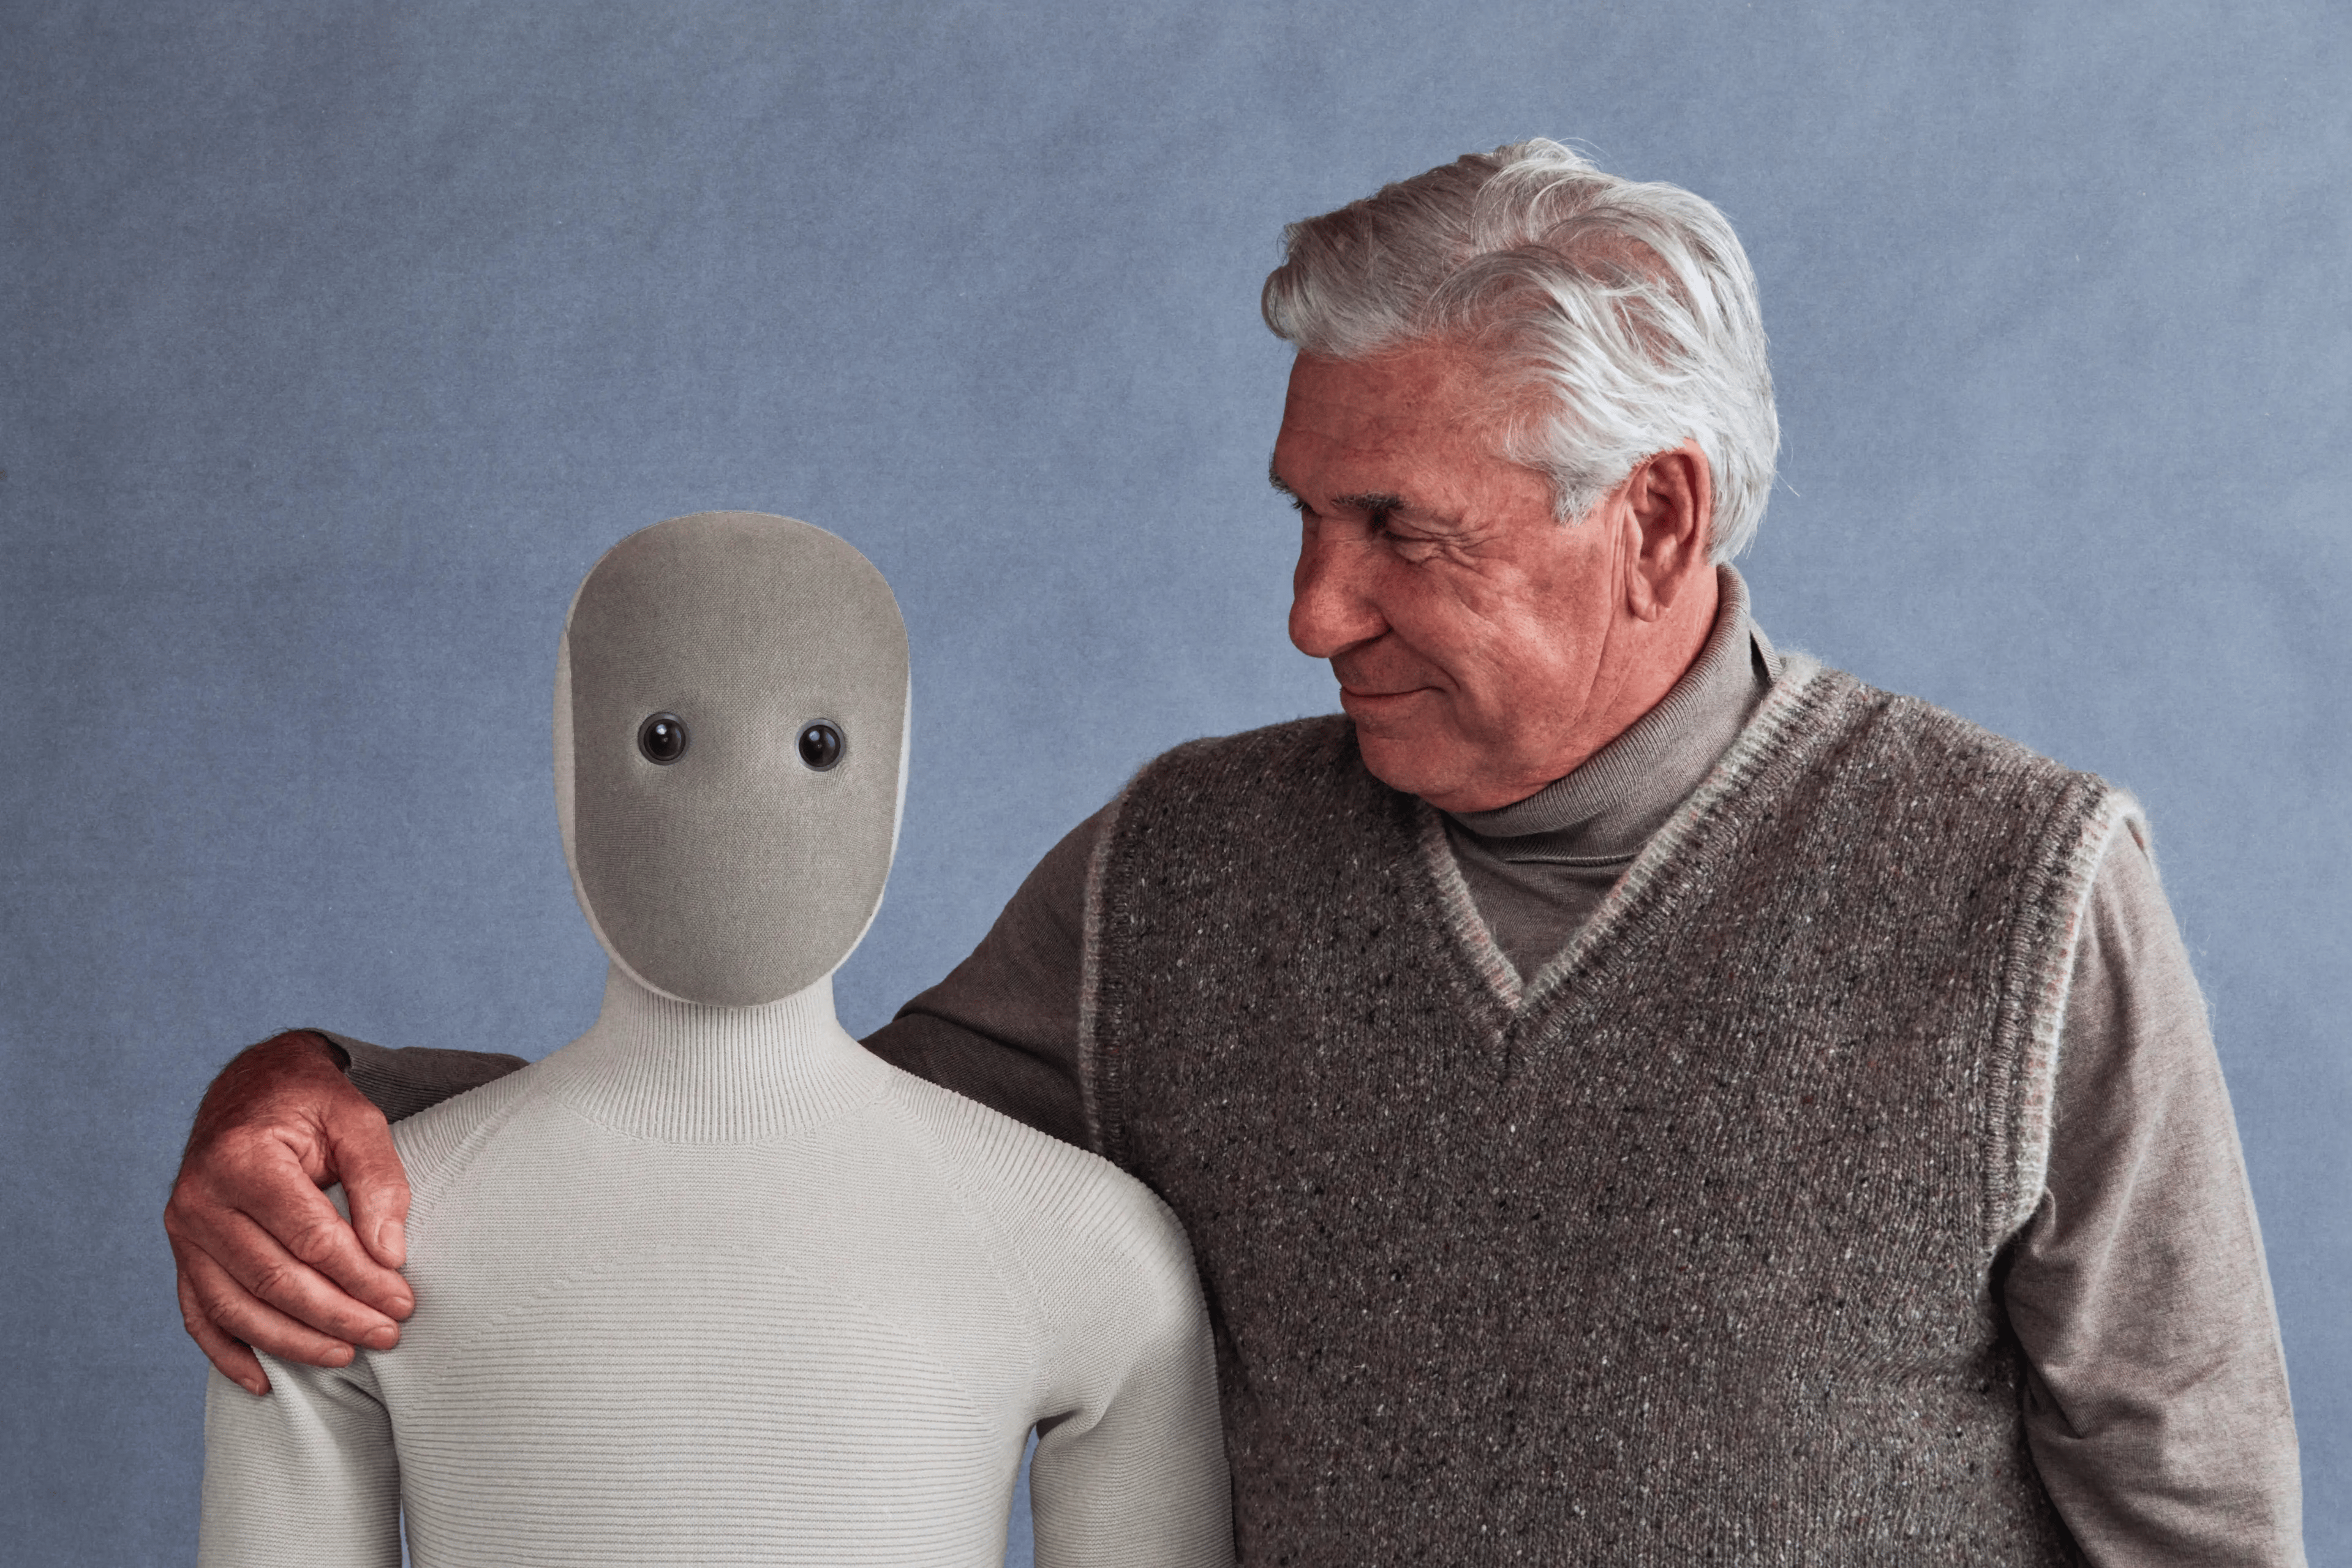
\includegraphics[width=2.5cm]{data/neo.png}
            };
            \node[inner sep=0pt, draw=black, label=below:\tiny{AlphaFold}] at (-0.5, -1.8) {
                \includegraphics[width=3cm]{data/alphafold.png}
            };
            \node[inner sep=0pt, draw=black, label=below:\tiny{AlphaZero}] at (3.8, -0.7) {
                \includegraphics[width=2.7cm]{data/chess.png}
            };
        }
        \only<2-4>{
			\node[circle, fill=babablue, minimum size=6cm] (ai) at (-3, 0) {};
			\node[text=white, anchor=north, align=center, font=\normalfont\linespread{0.9}\selectfont] at ($ (ai.north) - (0, 0.1) $) {Artificial\\intelligence};

            \node[
                anchor=north west,
                align=flush left,
                font=\small,
                text width=6cm,
                alt=<2>{text=black}{text=gray!40}
            ] (ai-text) at ($ (ai.north) + (3.5, 0.2) $) {
                    \textbf{Artificial intelligence:}\\Machines that solve tasks requiring some kind of (often human-like) intelligence.
            };

			\only<3->{
				\node[circle, fill=babablue!50!babared, minimum size=4.5cm, anchor=south] (ml) at ($ (ai.south) + (0, 0.05) $) {};
				\node[text=white, anchor=north, align=center, font=\normalfont\linespread{0.9}\selectfont] at ($ (ml.north) - (0, 0.1) $) {Machine\\learning};

				\node[
                    anchor=north west,
                    align=flush left,
                    font=\small,
                    text width=6cm,
                    alt=<3>{text=black}{text=gray!40}
                ] (ml-text) at ($ (ai-text.south west) - (0, 0) $) {\textbf{Machine learning:}\\Machines that learn to solve tasks by learning patterns from data};
			}
			\only<4->{
				\node[circle, fill=babared, minimum size=3cm, anchor=south] (dl) at ($ (ai.south) + (0, 0.1) $) {};
				\node[text=white, anchor=north, align=center, font=\normalfont\linespread{0.9}\selectfont] at ($ (dl.north) - (0, 0.1) $) {Deep\\learning};

				\node[
                    anchor=north west,
                    align=flush left,
                    font=\small,
                    text width=6cm
                ] (dl-text) at ($ (ml-text.south west) - (0, 0) $) {\textbf{Deep learning:}\\Machine learning approaches relying on artificial neural networks (inspired by the human brain)};
			}
        }

        \only<5->{
            \def\vsep{0.5}
            \def\hsep{0.65}
            \def\edgeopacity{0.5}

            \node[fill=gray!80, minimum width=4.5cm, minimum height=3.1cm, rounded corners=0.1cm, text=white, draw=black, font=\small, anchor=south, text depth=2.6cm] (model) at (0, -0.2) {
                Artificial neural network
            };

            \neuron[alt=<6>{fill=babagreen!60}{fill=babagreen}]{n00}{($ (model.south) + (0, 1.25) + (-2*\hsep, -2*\vsep+0.1) $)}
            \neuron[alt=<6>{fill=babagreen!40}{fill=babagreen}]{n01}{($ (n00) + (0, \vsep) $)}
            \neuron[alt=<6>{fill=babagreen!70!yellow}{fill=babagreen}]{n02}{($ (n00) + (0, 2*\vsep) $)}
            \neuron[alt=<6>{fill=babagreen!40!yellow}{fill=babagreen}]{n03}{($ (n00) + (0, 3*\vsep) $)}
            \neuron[alt=<6>{fill=babagreen!95}{fill=babagreen}]{n04}{($ (n00) + (0, 4*\vsep) $)}

            \neuron[alt=<6>{fill=babagreen!35!yellow}{fill=babagreen}]{n10}{($ (n00) + (\hsep, 0.5*\vsep) $)}
            \neuron[alt=<6>{fill=babagreen!55}{fill=babagreen}]{n11}{($ (n00) + (\hsep, 1.5*\vsep) $)}
            \neuron[alt=<6>{fill=babagreen!87!yellow}{fill=babagreen}]{n12}{($ (n00) + (\hsep, 2.5*\vsep) $)}
            \neuron[alt=<6>{fill=babagreen!92}{fill=babagreen}]{n13}{($ (n00) + (\hsep, 3.5*\vsep) $)}

            \neuron[alt=<6>{fill=babagreen!51}{fill=babagreen}]{n20}{($ (n00) + (2*\hsep, \vsep) $)}
            \neuron[alt=<6>{fill=babagreen!52!yellow}{fill=babagreen}]{n21}{($ (n00) + (2*\hsep, 2*\vsep) $)}
            \neuron[alt=<6>{fill=babagreen!81!yellow}{fill=babagreen}]{n22}{($ (n00) + (2*\hsep, 3*\vsep) $)}

            \neuron[alt=<6>{fill=babagreen!90}{fill=babagreen}]{n30}{($ (n00) + (3*\hsep, 1.5*\vsep) $)}
            \neuron[alt=<6>{fill=babagreen!41!yellow}{fill=babagreen}]{n31}{($ (n00) + (3*\hsep, 2.5*\vsep) $)}

            \neuron[alt=<6>{fill=babagreen!62!yellow}{fill=babagreen}]{n40}{($ (n00) + (4*\hsep, 2*\vsep) $)}

            \foreach \j in {0,...,4} {
                \draw[draw=black, opacity=\edgeopacity] ($ (model.west) - (0, 0.2175) $) -- (n0\j);
            }

            \foreach \j in {0,...,4} {
                \foreach \k in {0,...,3} {
                    \draw[draw=black, opacity=\edgeopacity] (n0\j) -- (n1\k);
                }
            }
            \foreach \j in {0,...,3} {
                \foreach \k in {0,...,2} {
                    \draw[draw=black, opacity=\edgeopacity] (n1\j) -- (n2\k);
                }
            }
            \foreach \j in {0,...,2} {
                \foreach \k in {0,...,1} {
                    \draw[draw=black, opacity=\edgeopacity] (n2\j) -- (n3\k);
                }
            }

            \draw[draw=black, opacity=\edgeopacity] (n30) -- (n40);
            \draw[draw=black, opacity=\edgeopacity] (n31) -- (n40);
            \draw[draw=black, opacity=\edgeopacity] (n40) -- ($ (model.east) - (0, 0.2175) $);
        }
        \only<5>{
            \node[circle, draw=black, fill=babagreen, minimum size=0.5cm] (neuron) at (0, -2.3) {};

            \node[anchor=east, font=\scriptsize] (x1) at ($ (neuron) - (0.75, -0.5) $) {$\text{input}_1$};
            \node[anchor=east, font=\scriptsize] (x2) at ($ (neuron) - (0.75, 0) $) {$\text{input}_2$};
            \node[anchor=east, font=\scriptsize] (x3) at ($ (neuron) - (0.75, 0.5) $) {$\text{input}_3$};

            \node[anchor=west, font=\scriptsize] (y) at ($ (neuron) + (0.75, 0) $) {$\text{output}$};

            \draw[-stealth] (x1) -- (neuron);
            \draw[-stealth] (x2) -- (neuron);
            \draw[-stealth] (x3) -- (neuron);
            \draw[-stealth] (neuron) -- (y);

            \node[font=\small] at ($ (neuron) + (0, 1.2) $) {
                Artificial neuron
            };
        }
        \only<6>{
            \node[anchor=east, inner sep=0pt, draw=black] (input) at ($ (model.west) - (1.5, 0.2175) $) {
                \includegraphics[width=2cm]{data/ladybug.png}
            };
            \node[font=\small, anchor=west] (output) at ($ (model.east) + (1.5, -0.2175) $) {
                Ladybug
            };
            \draw[-stealth] (input) -- ($ (model.west) - (0, 0.2175) $);
            \draw[-stealth] ($ (model.east) - (0, 0.2175) $) -- (output);
        }

    \end{tikzpicture}
\end{frame}


\newcommand{\pubmed}{
    \begin{tikzpicture}
        \begin{axis}[
            height=5.5cm,
            width=12cm,
            xlabel=\small{Year},
            ylabel=\small{Number of publications},
            ticklabel style={font=\small},
            axis lines=left,
            xtick pos=bottom,
            ytick pos=left,
            xmin=2000,
            xmax=2025,
            xtick={2000, 2005, 2010, 2015, 2020, 2025},
            xticklabels={2000, 2005, 2010, 2015, 2020, 2025}
        ]
            \addplot[
                babagreen,
                thick,
                mark=*
            ] table[col sep=comma, x=year, y=count] {data/pubmed.csv};
        \end{axis}
    \end{tikzpicture}
}
\newcommand{\classification}{
    \definecolor{MS}{HTML}{264653}
    \definecolor{AD}{HTML}{2a9d8f}
    \definecolor{PD}{HTML}{8ab17d}
    \definecolor{MDD}{HTML}{e9c46a}
    \definecolor{SCZ}{HTML}{f4a261}
    \definecolor{BP}{HTML}{e76f51}

    \def\marksize{3pt}
    \def\markopacity{0.5}

    \begin{tikzpicture}
        \begin{axis}[
            height=7cm,
            width=12cm,
            xlabel=\small{Year},
            ylabel=\small{Accuracy},
            ticklabel style={font=\small},
            xtick pos=bottom,
            ytick pos=left,
            xtick={2012, 2014, 2016, 2018, 2020, 2022},
            xticklabels={2012, 2014, 2016, 2018, 2020, 2022},
            xmin=2010,
            xmax=2023,
            ytick style={draw=none},
            ymajorgrids=true,
            ymin=50,
            ymax=100,
            legend style={
                font=\scriptsize,
                legend cell align=left,
                at={(rel axis cs: 0.02, 0.03)},
                anchor=south west
            },
            clip=false,
            x label style={yshift=5}
        ]
            \addplot[
                only marks,
                mark=*,
                mark size=\marksize,
                opacity=\markopacity,
                discard if not={diagnosis}{MS/HC},
                MS
            ] table [
                col sep=comma,
                x expr=\thisrow{year} + 0.5 * (rand - 0.5),
                y=accuracy
            ] {data/trial_lecture_data.csv};

            \addplot[
                only marks,
                mark=*,
                mark size=\marksize,
                opacity=\markopacity,
                discard if not={diagnosis}{AD/HC},
                AD
            ] table [
                col sep=comma,
                x expr=\thisrow{year} + 0.5 * (rand - 0.5),
                y=accuracy
            ] {data/trial_lecture_data.csv};

            \addplot[
                only marks,
                mark=*,
                mark size=\marksize,
                opacity=\markopacity,
                discard if not={diagnosis}{PD/HC},
                PD
            ] table [
                col sep=comma,
                x expr=\thisrow{year} + 0.5 * (rand - 0.5),
                y=accuracy
            ] {data/trial_lecture_data.csv};

            \addplot[
                only marks,
                mark=*,
                mark size=\marksize,
                opacity=\markopacity,
                discard if not={diagnosis}{MDD/HC},
                MDD
            ] table [
                col sep=comma,
                x expr=\thisrow{year} + 0.5 * (rand - 0.5),
                y=accuracy
            ] {data/trial_lecture_data.csv};

            \addplot[
                only marks,
                mark=*,
                mark size=\marksize,
                opacity=\markopacity,
                discard if not={diagnosis}{SCZ/HC},
                SCZ
            ] table [
                col sep=comma,
                x expr=\thisrow{year} + 0.5 * (rand - 0.5),
                y=accuracy
            ] {data/trial_lecture_data.csv};

            \addplot[
                only marks,
                mark=*,
                mark size=\marksize,
                opacity=\markopacity,
                discard if not={diagnosis}{BP/HC},
                BP
            ] table [
                col sep=comma,
                x expr=\thisrow{year} + 0.5 * (rand - 0.5),
                y=accuracy
            ] {data/trial_lecture_data.csv};

            \addlegendentry{Multippel sklerose (n=30)}
            \addlegendentry{Alzheimers sykdom (n=139)}
            \addlegendentry{Parkinsons sykdom (n=19)}
            \addlegendentry{Depresjon (n=3)}
            \addlegendentry{Schizofreni (n=29)}
            \addlegendentry{Bipolar lidelse (n=3)}

            \addplot[thick, MS] coordinates {
                (2010, 94.54) (2023, 94.54)
            };
            \node[text=MS, font=\tiny\bfseries, anchor=west, inner sep=2pt] at (axis cs: 2023, 94.54) {94.14\%};
            \addplot[thick, AD] coordinates {
                (2010, 92.92) (2023, 92.92)
            };
            \node[text=AD, font=\tiny\bfseries, anchor=west, inner sep=2pt] at (axis cs: 2023, 92.92) {92.92\%};
            \addplot[thick, PD] coordinates {
                (2010, 91.4) (2023, 91.4)
            };
            \node[text=PD, font=\tiny\bfseries, anchor=west, inner sep=2pt] at (axis cs: 2023, 91.4) {91.91\%};
            \addplot[thick, MDD] coordinates {
                (2010, 85.11) (2023, 85.11)
            };
            \node[text=MDD, font=\tiny\bfseries, anchor=west, inner sep=2pt] at (axis cs: 2023, 85.11) {85.11\%};
            \addplot[thick, SCZ] coordinates {
                (2010, 82.18) (2023, 82.18)
            };
            \node[text=SCZ, font=\tiny\bfseries, anchor=west, inner sep=2pt] at (axis cs: 2023, 82.18) {82.18\%};
            \addplot[thick, BP] coordinates {
                (2010, 67.66) (2023, 67.66)
            };
            \node[text=BP, font=\tiny\bfseries, anchor=west, inner sep=2pt] at (axis cs: 2023, 67.66) {67.66\%};
        \end{axis}
    \end{tikzpicture}
}

\begin{frame}{Artificial intelligence and clinical neuroimaging}
    \begin{tikzpicture}
        \node[draw=black] at (-7, -3.25) {};
        \node[draw=black] at (7, 3.25) {};

        \only<1>{
            \node[draw=black, inner sep=0pt] at (0, 0.2) {
                \includegraphics[width=10cm]{data/mckinsey.png}
            };
            \node[anchor=south, font=\tiny, text width=10.5cm, align=flush center] at (0, -3.5) {
                The state of AI 2025, McKinsey \& Company
            };
        }
        \only<2>{
            \node[draw=black, inner sep=0pt] at (0, 0.2) {
                \includegraphics[width=12cm]{data/mit.png}
            };
            \node[anchor=south, font=\tiny, text width=10.5cm, align=flush center] at (0, -3.5) {
                NANDA, MIT (2025). State of AI in Business 2025. \textit{Preprint at https://www.artificialintelligence-news.com/wp-content/uploads/2025/08/ai\_report\_2025.pdf}
            };
        }

        \only<3>{
            \node[] at (-0.65, 0.2) {
                \pubmed
            };
            \node[anchor=south, font=\tiny, text width=10.5cm, align=flush center] at (0, -3.5) {
                Publications containing "(neuroimaging OR clinical neuroscience) AND (artificial intelligence OR deep learning)" from https://pubmed.ncbi.nlm.nih.gov
            };
        }
        \only<4-5>{
            \mriside{-4.5}{0}{1.5cm}{data/mri_sagittal.png}
            \cnnarrow{(input.east)}{($ (input.center) + (3, 0) $)}{black}
            \cnn{-2.7}{0}{0.1}{0.15}{babagreen}{1}
        }
        \only<4>{
            \node[anchor=west, align=left, font=\small\linespread{0.9}\selectfont] (output) at (3.55, 0){Clinically\\relevant\\prediction};
            \cnnarrow{($ (output.west) - (1, 0) $)}{($ (output.west) + (0.1, 0) $)}{black}
        }
        \only<5>{
            \node[anchor=west, align=left, font=\small\linespread{0.9}\selectfont] (output1) at ($ (3.55, 0) + (0, 0.5) $) {Patient};
            \node[anchor=west, align=left, font=\small\linespread{0.9}\selectfont] (output2) at ($ (3.55, 0) - (0, 0.5) $) {Healthy\\control};
            \cnnarrow{($ (output1.west) - (1, 0.5) $)}{($ (output1.west) + (0.1, 0) $)}{black}
            \cnnarrow{($ (output2.west) - (1, -0.5) $)}{($ (output2.west) + (0.1, 0) $)}{black}
        }
        \only<6>{
            \node[] at (0, 0) {
                \classification
            };
        }
        \only<7>{
            \node[] at (0, 0) {
                AI adoption
            };
        }
    \end{tikzpicture}
\end{frame}

